\section{Results}\label{sec:results}
The completed evidence consists of three distinct components: a frozen five-seed QSNN-v3 validation campaign, a seed-42 paired native-timestamp attack comparison, and a seed-42 four-model packet-grid study. We report their denominators and computational definitions separately. Percentages below are conditional on the stated split and, for ASR, the stated clean-correct population; no result is reconstructed for an uncompleted experiment.

\subsection{Clean validation of the hybrid classifier}
The frozen QSNN-v3 configuration achieves 97.2720\% $\pm$ 0.2119\% validation accuracy and a reported macro-F1 of 97.2736\% $\pm$ 0.2119\% across five training seeds. Individual accuracies are 97.06\%, 97.28\%, 97.52\%, 97.44\% and 97.06\% for seeds 42, 123, 777, 2026 and 6543, respectively; the descriptive span is 0.46 percentage points. The preserved SNN validation reference has 98.1320\% $\pm$ 0.2407\% accuracy, giving a descriptive QSNN-minus-SNN difference of -0.8600 percentage points. A matched validation-F1 comparison is unavailable.

The five hybrid runs share one pretrained seed-42 frontend and one 55,000/5,000 training/validation split. The architecture and training configuration were frozen after seed-42 development. Thus, the sample standard deviation measures subsequent training variation conditional on shared pretraining and data, rather than five independently pretrained pipelines. The selected epochs are 37, 24, 40, 38 and 40. The seed-42 process was externally terminated during epoch 38; its saved epoch-37 checkpoint was reloaded and evaluated for the reported result.

The seed-42 wide4 classical frontend reaches 97.80\% validation accuracy with 38,122 parameters, while its selected hybrid continuation reaches 97.06\% with 40,762 parameters. The 0.74-point accuracy difference and 2,640 added parameters are descriptive: differing training stages and budgets prevent attribution to an isolated circuit component. All final QSNN clean results are validation results; the official test partition was not accessed. The campaign establishes an accurate implemented hybrid victim, rather than a quantum accuracy advantage.

Figure~\ref{fig:matched}a shows the individual runs and their conditional mean and sample standard deviation. Table~\ref{tab:validation} gives the selected checkpoint epochs; full per-run training records are retained in the supplement.
\begin{table}[t]\centering
\caption{QSNN-v3 validation on the same 5,000 examples.}\label{tab:validation}
\small\begin{tabularx}{\linewidth}{L C C}\toprule
\textbf{Seed} & \textbf{Accuracy (\%)} & \textbf{Epoch}\\\midrule
42 & 97.06 & 37\\
123 & 97.28 & 24\\
777 & 97.52 & 40\\
2026 & 97.44 & 38\\
6543 & 97.06 & 40\\\midrule
Mean $\pm$ SD & $97.272\pm0.212$ & ---\\\bottomrule
\end{tabularx}
\vspace{3pt}\begin{minipage}{\linewidth}\footnotesize
All seeds reuse one pretrained frontend and one split. Reported macro-F1 is $97.2736\%\pm0.2119\%$ [R1].
\end{minipage}\end{table}

\subsection{Matched timestamp attacks}
All timestamp conditions reuse 100 seed-42 validation examples, ten per class, that both QSNN-v3 and the compact SNN classify correctly before attack. One success therefore equals one ASR percentage point. PGD uses 21 candidate evaluations, 41 attack-internal forwards and 20 backwards; TEMP uses Q forwards/candidates and no backwards. Candidate, forward-pass and elapsed-time matching consequently answer different computational questions. The two verification forwards per new record are excluded from attack timing.

Under 21-candidate matching, QSNN-v3 PGD succeeds on 3/100 examples at both duration-scaled budgets, $\epsilon_f$ = 0.05 and 0.10; TEMP succeeds on 4/100 and 3/100. Matching 41 forwards produces the same outcomes. Elapsed-time calibration selects Q = 4,000 for QSNN-v3 and Q = 1,600 for SNN, with median TEMP/PGD runtime ratios of 0.978 and 1.083. Under this calibration TEMP succeeds on 4/100 and 5/100 QSNN examples, compared with PGD's 3/100 at each budget. Thus the two-example numerical TEMP advantage at 10\% occurs under elapsed-time matching and disappears under the two access definitions.

The paired counts delimit this contrast. At 5\% the QSNN attacks share three successes, with one TEMP-only success and 96 failures of both attacks. At 10\% under access matching, both attacks break the same three examples. At 10\% under elapsed-time matching, three are broken by both, two only by TEMP and 95 by neither. The respective exact paired p-values are 1, 1 and 0.5. No matched condition establishes significant TEMP superiority, and nonsignificance does not prove attack equivalence.

The paired comparison is driven by discordant examples, not by treating the two ASRs as independent proportions. At the 10\% budget under elapsed-time calibration, the two TEMP-only failures account for the entire numerical difference; there are no PGD-only failures. The exact paired test therefore remains inconclusive at $p=0.5$. At the same budget under candidate or forward matching, the attacks fail on exactly the same three examples. These observations identify a budget-dependent numerical contrast within this fixed population, without establishing a generally stronger attack.

The compact SNN has no successes for either attack under candidate or forward matching at either budget. Elapsed-time matching yields no successes at 5\%, and 0/100 PGD versus 1/100 TEMP at 10\% (exact paired p = 1). These finite, joint-correct, single-seed observations demonstrate specific hybrid failures but neither population-wide robust accuracy nor general hybrid-versus-SNN robustness. Supporting material retains the original fixed-budget rows, reported bootstrap intervals and report-specific distortion diagnostics separately.

Figure~\ref{fig:matched}b--d visualizes all three computational controls, and Table~\ref{tab:timestamp} reports their exact counts. These repeated conditions do not add independent test subjects.

\begin{table*}[t]
\centering
\caption{Matched timestamp attacks on 100 common clean-correct validation examples. Success counts also equal ASR percentages.}\label{tab:timestamp}
\small
\setlength{\tabcolsep}{4pt}
\renewcommand{\arraystretch}{1.16}
\begin{tabularx}{\linewidth}{L C C C C C}
\toprule
\textbf{Matching} & \textbf{Model} & \textbf{$\epsilon_f$ \%} & \textbf{PGD n} & \textbf{TEMP n} & \textbf{Exact p}\\
\midrule
21 candidates & SNN & 5 & 0 & 0 & 1\\
21 candidates & SNN & 10 & 0 & 0 & 1\\
21 candidates & QSNN & 5 & 3 & 4 & 1\\
21 candidates & QSNN & 10 & 3 & 3 & 1\\
41 forwards & SNN & 5 & 0 & 0 & 1\\
41 forwards & SNN & 10 & 0 & 0 & 1\\
41 forwards & QSNN & 5 & 3 & 4 & 1\\
41 forwards & QSNN & 10 & 3 & 3 & 1\\
Elapsed time & SNN & 5 & 0 & 0 & 1\\
Elapsed time & SNN & 10 & 0 & 1 & 1\\
Elapsed time & QSNN & 5 & 3 & 4 & 1\\
Elapsed time & QSNN & 10 & 3 & 5 & 0.5\\
\bottomrule
\end{tabularx}
\vspace{3pt}
\begin{minipage}{\linewidth}\footnotesize Seed 42 validation examples; successes n are also ASR percentages. Exact paired p-values were recalculated from report discordant counts. Source: [R3].\end{minipage}
\end{table*}

\begin{figure*}[t]
\centering
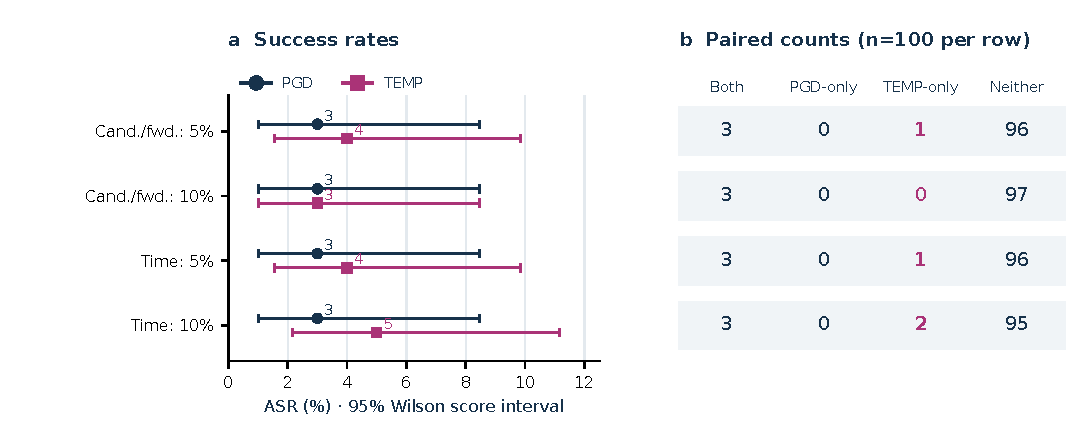
\includegraphics[width=\textwidth]{figures/fig02_matched_evaluation.pdf}
\caption{QSNN validation and paired timestamp attacks. (a) Five training seeds yield 97.272\% $\pm$ 0.212 percentage points (mean $\pm$ sample SD) on 5,000 validation examples. All runs share a split and pretrained frontend. (b--d) PGD/TEMP successes on the same 100 jointly clean-correct validation examples (seed 42); counts equal ASR percentages. Conditions match candidates, attack forwards, or calibrated elapsed time. Time matching uses TEMP Q=4,000 (QSNN) and 1,600 (SNN), with median TEMP/PGD timing ratios 0.978 and 1.083. All exact paired McNemar comparisons are nonsignificant; the largest discordance is b=0, c=2 (p=0.5). Backward costs are not equated by access matching. Sources: [R1, R3].}\label{fig:matched}
\end{figure*}

\subsection{Controlled packet-grid comparison}
The four-model grid study is separate from the timestamp experiment. It uses ten equal-event-count bins and amplitude-preserving packet retiming, with the same local training recipe, split, seed 42 and validation-selected checkpoint rule across architectures. Clean accuracy uses all 10,000 official-test examples. Each representation has its own frozen manifest of the first 1,000 examples correctly classified by all four models, selected from joint-correct pools of 9,522 binary and 9,495 integer examples. These common manifests are reused within representation for the two completed budgets, $B_\infty$ = 1 bin and B0 = 200 retimed packets.

On binary grids the custom SNN has 100.0\% and 99.5\% ASR under $B_\infty$ and B0, respectively. ConvNet has 1.9\% and 1.2\%, spiking ResNet18 has 0.1\% and 0.0\%, and VGGSNN has 0.0\% in both cells. Their full-test clean accuracies are 97.99\%, 96.90\%, 98.61\% and 99.21\%. On integer grids the corresponding ASR pairs are 99.9\%/98.0\%, 0.6\%/1.1\%, 0.2\%/0.1\% and 0.0\%/0.0\%, with clean accuracies of 98.14\%, 96.58\%, 98.12\% and 99.30\%. Each 0.1 ASR point represents one success among 1,000 attacked examples; the table gives all sixteen completed cells.

The largest reference-model ASR is descriptively 98.1 and 98.3 percentage points below the custom SNN for the binary budgets, and 99.3 and 96.9 points below it for the integer budgets. The integer-grid comparison supplies a particularly clear diagnostic: the custom SNN and spiking ResNet18 differ by only $0.02$ percentage points in clean test accuracy, but by $99.7$ and $97.9$ points in ASR under the two completed budgets. Similar clean accuracy therefore does not summarize the failure profile under this attack recipe. The source of the contrast remains unresolved, because a common recipe does not guarantee comparable optimization strength across architectures. In particular, zero observed successes should be read as failure of the evaluated attack on the selected examples, rather than as a robustness certificate \cite{athalye2018obfuscated,croce2020reliable}.

The source report states that every attack cell passed independent raw-data reconstruction and prediction audit. Common inputs and settings support a local architecture comparison without identifying the cause of the ASR gap. The campaign has one seed and two budgets; an unresolved B0 penalty discrepancy (5 attributed to the implementation by the report versus 10 in the reference paper) also limits replication claims. These local measurements must remain separate from published-reference tables, historical custom-SNN campaigns and the native-timestamp results.

Figure~\ref{fig:grid} shows the full 0--100\% outcome range and explicitly labeled control expansions. Table~\ref{tab:grid} gives every completed attack cell.

\begin{table*}[t]
\centering
\caption{Controlled four-model packet-grid results. Clean accuracy and ASR use different stated populations.}\label{tab:grid}
\small
\setlength{\tabcolsep}{4pt}
\renewcommand{\arraystretch}{1.16}
\begin{tabularx}{\linewidth}{L L C C C}
\toprule
\textbf{Grid} & \textbf{Architecture} & \textbf{Clean test \%} & \textbf{ASR $B_\infty$ = 1 \%} & \textbf{ASR $B_0$ = 200 \%}\\
\midrule
Binary & Custom SNN & 97.99 & 100.0 & 99.5\\
Binary & ConvNet & 96.90 & 1.9 & 1.2\\
Binary & Spiking ResNet18 & 98.61 & 0.1 & 0.0\\
Binary & VGGSNN & 99.21 & 0.0 & 0.0\\
Integer & Custom SNN & 98.14 & 99.9 & 98.0\\
Integer & ConvNet & 96.58 & 0.6 & 1.1\\
Integer & Spiking ResNet18 & 98.12 & 0.2 & 0.1\\
Integer & VGGSNN & 99.30 & 0.0 & 0.0\\
\bottomrule
\end{tabularx}
\vspace{3pt}
\begin{minipage}{\linewidth}\footnotesize Clean accuracy uses the complete 10,000-example official test set. ASR uses a separate frozen 1,000-example joint-correct manifest per representation. These are local measurements, not values copied from \cite{yu2026}. Source: [R4].\end{minipage}
\end{table*}

\begin{figure*}[t]
\centering
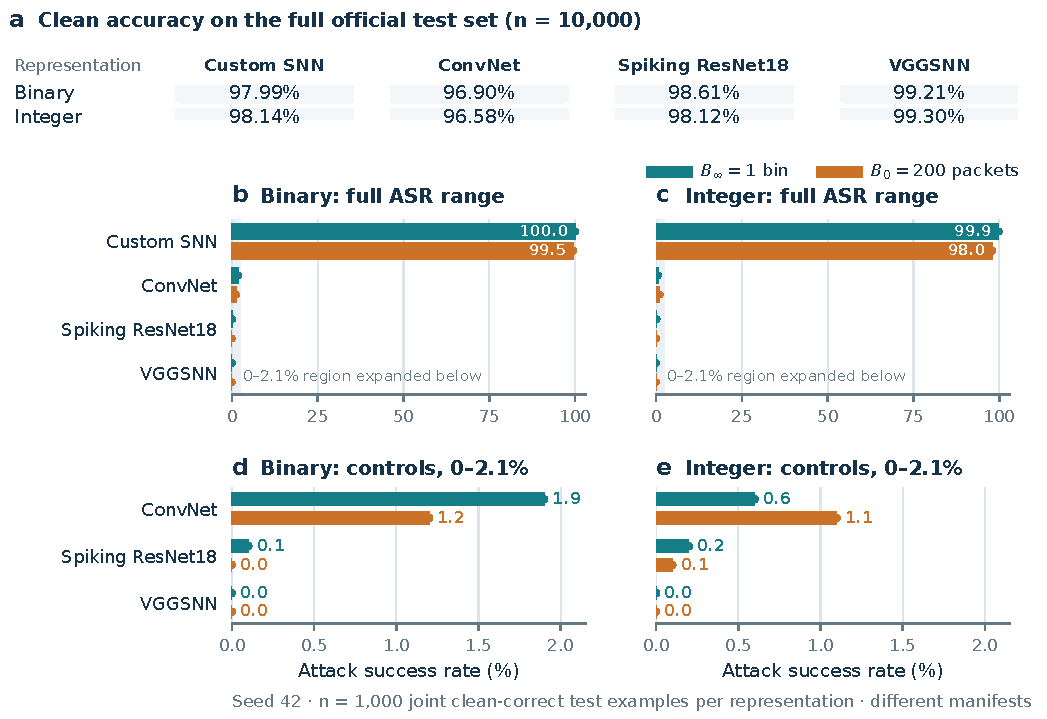
\includegraphics[width=\textwidth]{figures/fig03_grid_comparison.pdf}
\caption{Controlled local packet-retiming results (seed 42). (a) Clean accuracy uses all 10,000 official-test examples. (b,c) Full-range ASR under the two completed budgets; (d,e) declared expansions show the three controls at 0--2.1\%. Each attack cell uses 1,000 joint clean-correct test examples, so 0.1 percentage point is one success. Manifests are shared within each representation and differ between binary and integer. The local training and attack recipe is held constant across architectures. These single-seed, attack-specific results do not establish an architecture-independent ranking. The grid Custom SNN differs from the timestamp SNN. Source: controlled four-model report [R4].}\label{fig:grid}
\end{figure*}
